%\usepackage{graphicx}

\chapter{Design}\label{ch:design}

\section{User Modelling}

To determine the different user types that users of our system will be able to select from, we will perform a survey spanning a variety of different topographies as mentioned in the Background Research section. If the survey results do not yield any significant preference patterns for users, we can fallback to asking users to complete a short version of our survey upon login to our system. This way, we can still generate a list of preferences for each individual user - the only tradeoff is less convenience for the user.

\begin{itemize}
  \item Discuss the survey and analyze results?
\ldots
\end{itemize}

\section{System Architecture}

\begin{center}
  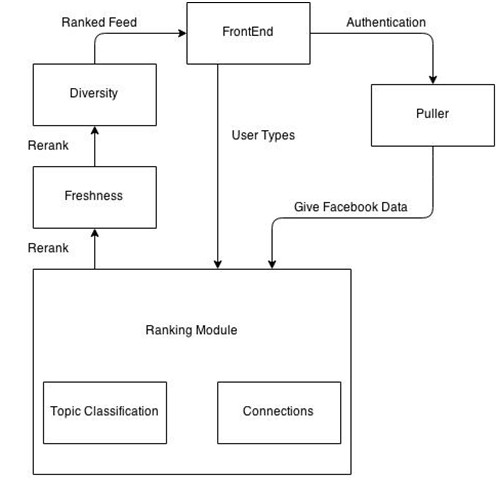
\includegraphics[scale=0.6]{images/blockdiagram.jpg}
  \captionof{figure}{Block Diagram}
\end{center}

Figure 3.1 provides a general overview of our implementation plan. It is a block diagram of our system. 

In our design, we will have a front end module which will be the website that is seen be the user. The website will have a login screen for user authentication which will allow us to pull the data from their Facebook feed. This is the job of the puller module.  The user will be given a couple of options of which user type that they think they are. The associated weights from the user types will be brought into the ranking module which contains two algorithms, one for topic classification and one for connections. The puller module will pull the feed in data into this ranking module which will rank the feed using the total scores from the topic classification, connection module and the assigned weights of the user types that came from the website or front end. To do topic classification we will look at the user's posts and try to generalise the topic based on what they have written. We will use the method proposed by Szo~\cite{szomszor2008semantic} to do topic classification.
The connections module will simply look at how often the user has interacted with the person who posted that item and give a score based on that. 

After the scores have been assigned to each post,  the feed will be ranked on the score and passed over to the freshness module. We will use Aga's~\cite{Aga2014} method and assign a decay factor to feeds that are not as recent. This feed will be reranked based on the new scores and passed over to the diversity module. In this module, we will rerank the feed and add a negative score to consecutive posts of the same type. Lastly, the newly ranked feed will be displayed in the frontend in front of the user.

We plan to use nodejs to do the whole project due to its flexibility and adaptability. We will use some written nodejs API's in order to interact with the Facebook API. 
